\documentclass[a4paper,11pt]{article}
\usepackage{tikz}
\tikzset{%
  every neuron/.style={
    circle,
    draw,
    minimum size=1cm
  },
  neuron missing/.style={
    draw=none, 
    scale=4,
    text height=0.333cm,
    execute at begin node=\color{black}$\vdots$
  },
}

\begin{document}
\begin{center}
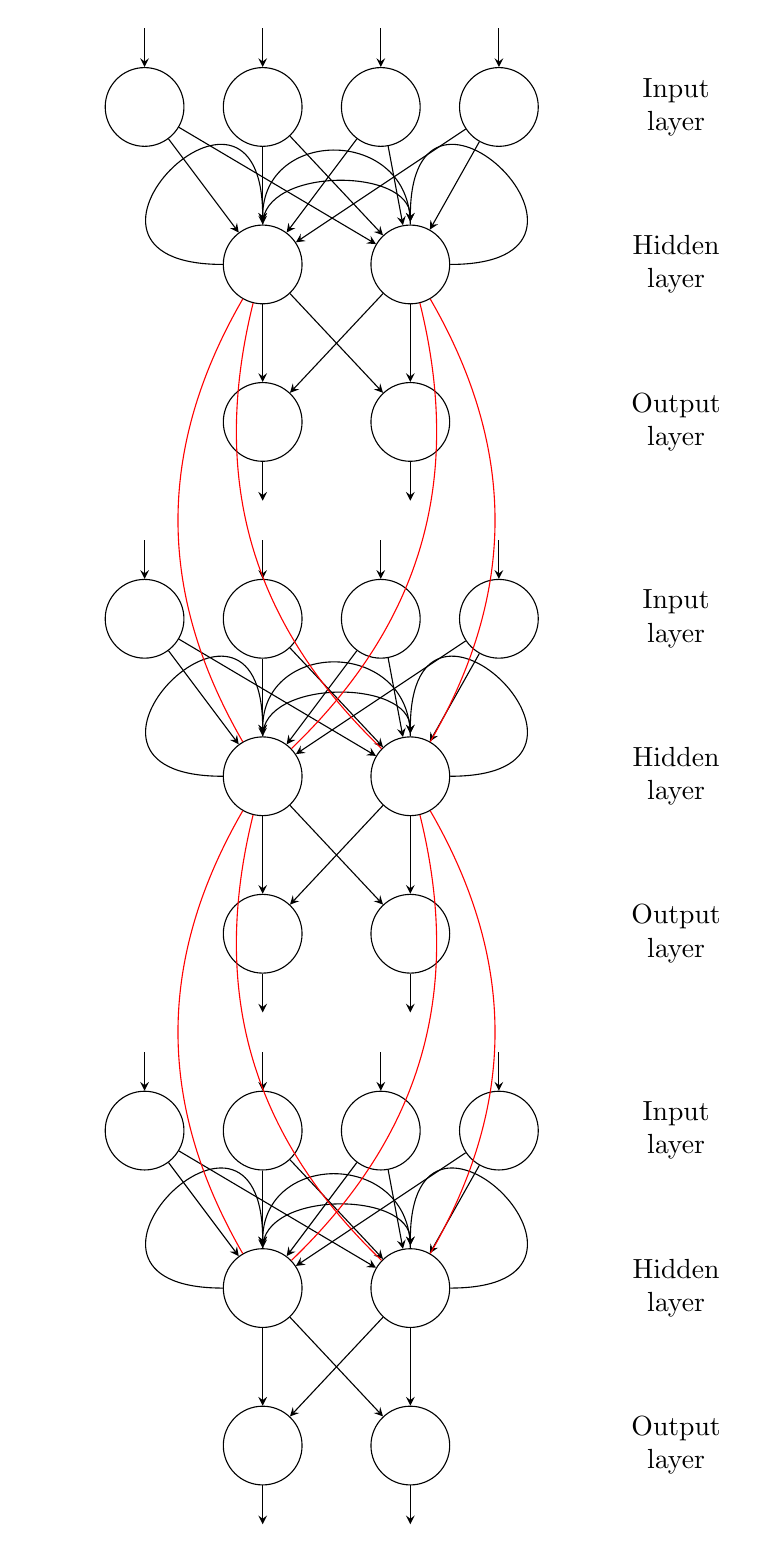
\begin{tikzpicture}[
   % swap the unit vectors
   x={(0,-1cm)},
   y={(1.5cm,0)},
   >=stealth,
   ]
\foreach [count=\xx] \X in {0,6.5,13}{
\foreach \m/\l [count=\y] in {1,2,3,4}
  \node [every neuron/.try, neuron \m/.try] (input-\m-\xx) at (0+\X,2.5-\y) {};

\foreach \m [count=\y] in {1,2}
  \node [every neuron/.try, neuron \m/.try ] (hidden-\m-\xx) at (2+\X,2-\y*1.25) {};

\foreach \m [count=\y] in {1,2}
  \node [every neuron/.try, neuron \m/.try ] (output-\m-\xx) at (4+\X,2-\y*1.25) {};

\foreach \l [count=\i] in {1,2,3,n}
  \draw [<-] (input-\i-\xx) -- ++(-1,0);
%    node [above, midway] {};

%\foreach \l [count=\i] in {1,n}
%  \node [above] at (hidden-\i-\xx.north) {};

\foreach \l [count=\i] in {1,n}
  \draw [->] (output-\i-\xx) -- ++(1,0);
%    node [above, midway] {};

\foreach \i in {1,...,4}
  \foreach \j in {1,...,2}
    \draw [->] (input-\i-\xx) -- (hidden-\j-\xx);

\foreach \i in {1,...,2}
  \foreach \j in {1,...,2}
    \draw [->] (hidden-\i-\xx) -- (output-\j-\xx);

\draw[->,shorten >=1pt] (hidden-1-\xx) to [out=0,in=90,loop,looseness=8.8] (hidden-1-\xx);
\draw[->,shorten >=1pt] (hidden-2-\xx) to [out=180,in=90,loop,looseness=8.8] (hidden-2-\xx);

\draw[->,shorten >=1pt] (hidden-1-\xx) to [out=90,in=90,loop,looseness=1.7] (hidden-2-\xx);
\draw[->,shorten >=1pt] (hidden-2-\xx) to [out=90,in=90,loop,looseness=1] (hidden-1-\xx);


\foreach \l/\txt [count=\x from 0] in {Input/input, Hidden/hidden, Output/output}
  \node [align=center] at (\txt-1-\xx-|+0,3) {\l \\ layer};
}% end of outer foreach


\foreach [evaluate=\i as \j using int(\i+1)] \i in {1,2}
{
  \draw [red] (hidden-1-\i) to[bend left] (hidden-1-\j);
  \draw [red] (hidden-1-\i) to[bend left] (hidden-2-\j);
  \draw [red] (hidden-2-\i) to[bend right] (hidden-1-\j);
  \draw [red] (hidden-2-\i) to[bend right] (hidden-2-\j);


}
\end{tikzpicture}
\end{center}
\end{document}